\chapter{Mechanical Design}
\section{Introduction}
The robot meets the design specification shown in Table \ref{tab:roborodentia_reqs}. It consists of four subassemblies: the base platform, shooting mechanism, ball hopper, and control unit. Each section was first modeled in SolidWorks, an industry-standard solid modeling CAD program. The designed parts were then fabricated using a laser cutter or 3D printer and assembled with metric hardware. Figures \ref{fig:render_isometric} through \ref{fig:render_right} show standard view renders of the robot.

\begin{table}[h]
	\caption{Roborodentia Mechanical Requirements}
	\begin{tabular}{cp{5in}}
		\hline 
		& Contest Requirement \\ 
		\hline 
		1 & \ssp Maximum footprint of 12" x 14" or smaller at start of match but may expand up to 14" x 17" during match. \\ 
		\hline 
		2 & \ssp Maximum height of 14" at start of match but no restriction during match. \\ 
		\hline 
		3 & Robot may not disassemble into multiple parts. \\ 
		\hline 
		4 & Robot may not be airborne. \\ 
		\hline 
		5 & Shooting mechanisms may not accelerate balls past 50 feet per second. \\ 
		\hline 
	\end{tabular} 
	\label{tab:roborodentia_reqs}
\end{table}

\begin{figure}[H]   % [h] means here
	\centering 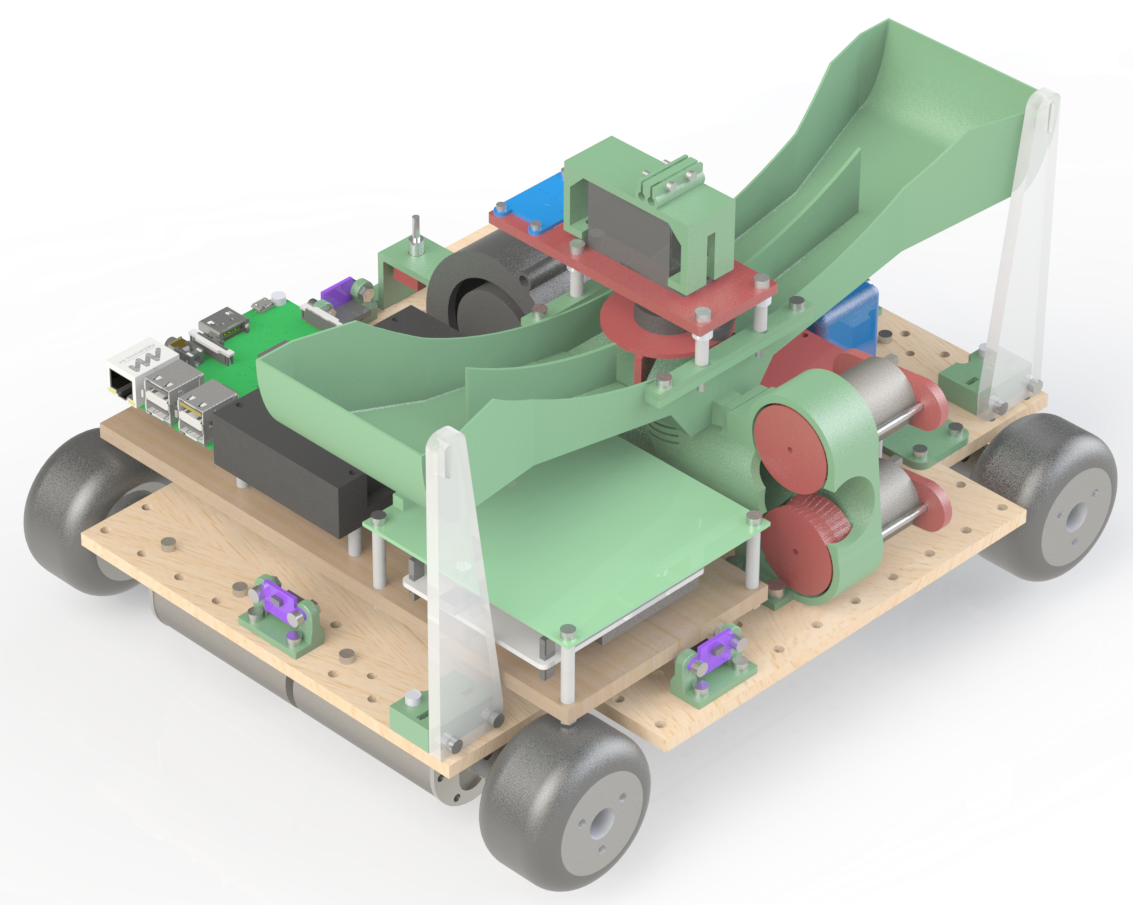
\includegraphics[width=6in, height=3.85in, keepaspectratio]{figures/render_isometric.png}
	\caption{Full Robot Render -- Isometric View}\label{fig:render_isometric}
\end{figure}
\begin{figure}[H]   % [h] means here
	\centering 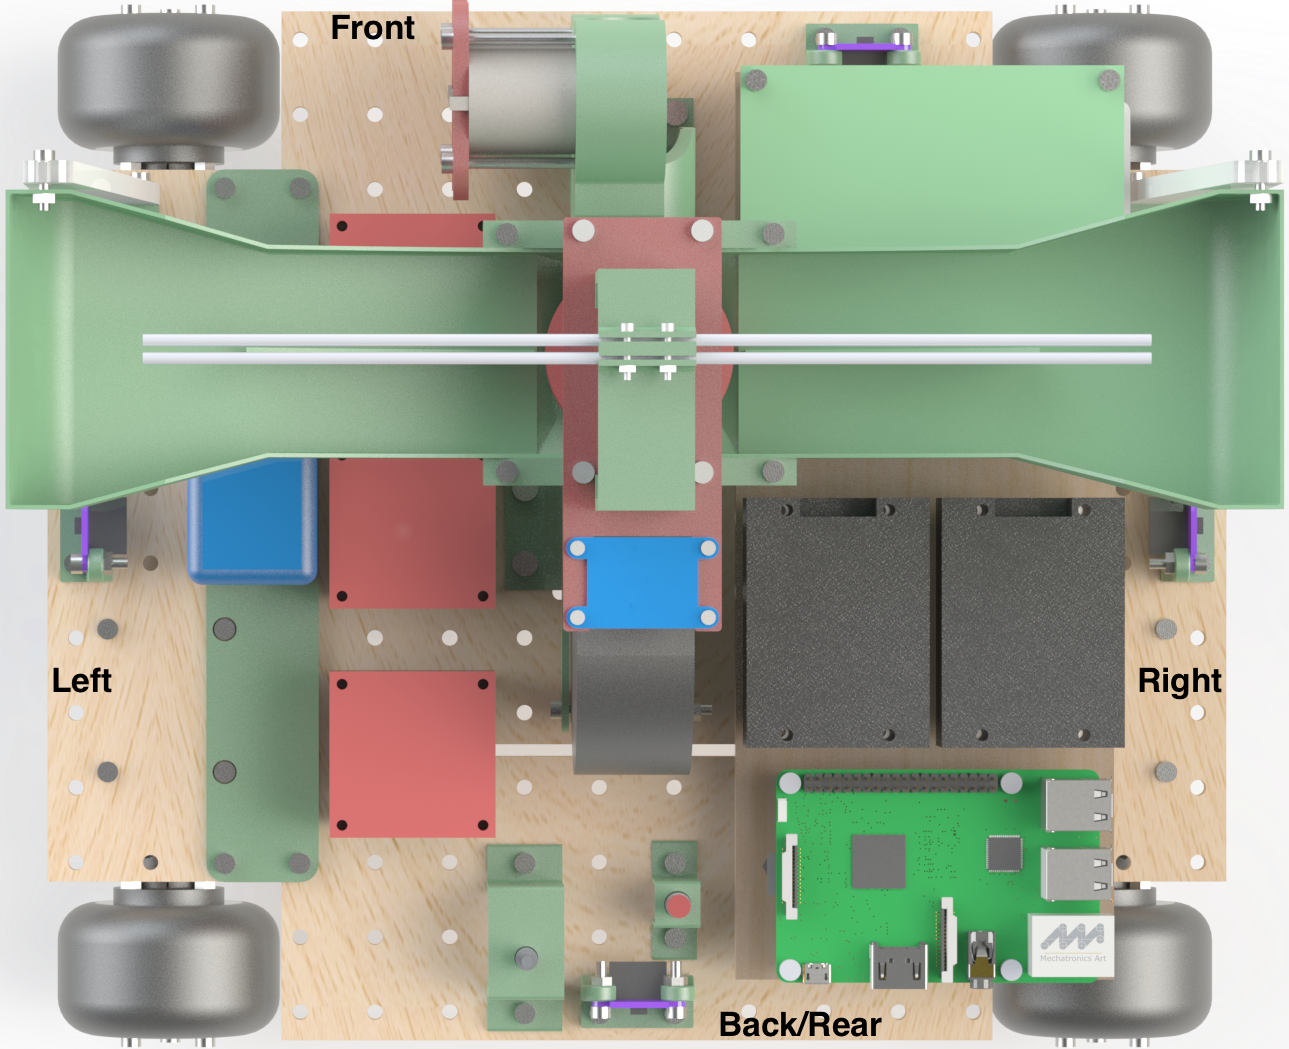
\includegraphics[width=6in, height=3.85in, keepaspectratio]{figures/render_top.png}
	\caption{Full Robot Render -- Top View}	\label{fig:render_top}
\end{figure}
\begin{figure}[H]   % [h] means here
	\centering 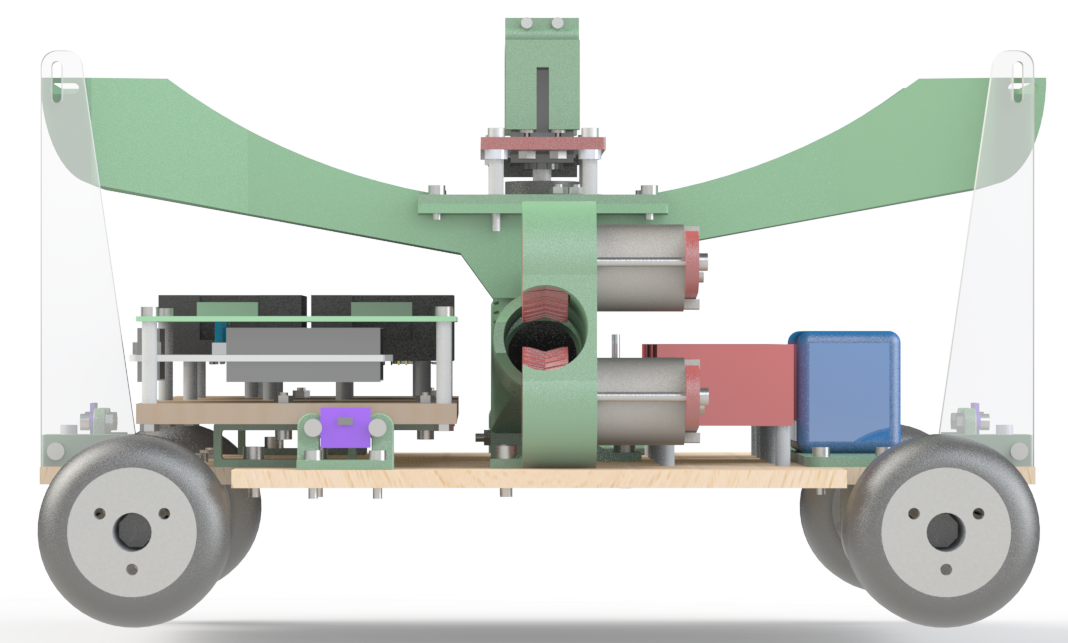
\includegraphics[width=6in, height=3.85in, keepaspectratio]{figures/render_front.png}
	\caption{Full Robot Render -- Front View}	\label{fig:render_front}
\end{figure}
\begin{figure}[H]   % [h] means here
	\centering 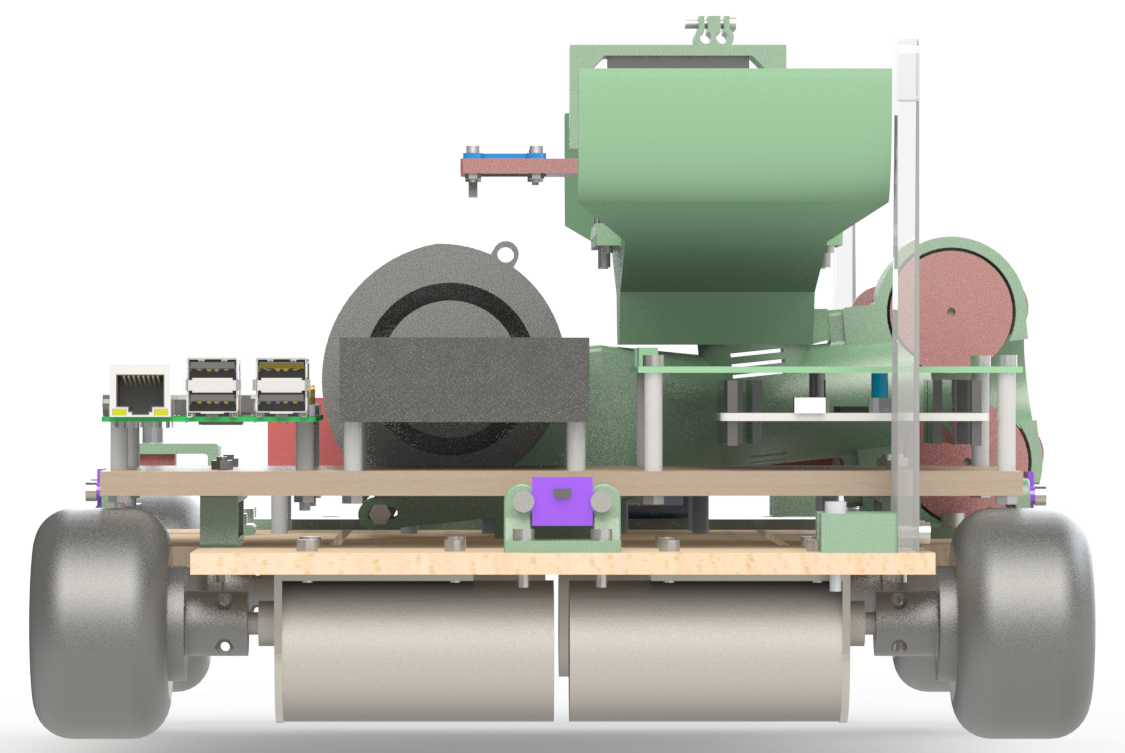
\includegraphics[width=6in, height=3.85in, keepaspectratio]{figures/render_right.png}
	\caption{Full Robot Render -- Right View}	\label{fig:render_right}
\end{figure}

\section{Base Platform}

\section{Shooting Mechanism}
The shooting mechanism naturally takes inspiration from the official Nerf Rival Blaster toys since the manufacturer specifically optimized them to fire Nerf Rival balls in a way similar to baseball pitching machines. Figure \ref{fig:shooter_explode} shows an exploded view of the subassembly while Figure \ref{fig:shooter_top} displays the top view. The mechanism consists of two sections: the \textbf{barrel} (left green part in Figure \ref{fig:shooter_explode}) and the \textbf{wheel housing} (right green part in Figure \ref{fig:shooter_explode}). Both parts were fabricated using a fused deposition modeling (FDM) 3D printer as the geometries are highly complex. Therefore, the shooting mechanism consists of two separate components versus a unibody design to allow each half to be fabricated with optimal print direction, strength, and finish quality. 

The \textbf{barrel} directs balls from the \textbf{ball hopper} to the \textbf{wheel housing}. First, the ball enters the barrel through a vertical chute by force of gravity. As the ball falls into the barrel, a high-pressure centrifugal (or blower fan) attached at the back of the barrel pushes it into the wheel housing inlet. As seen in Figure \ref{fig:shooter_xsec}, the barrel slightly narrows in the area behind the top chute to prevent the ball from rolling backwards towards the blower fan. A loft feature creates a smooth transition between the rectangular fan connection and the circular barrel. The foam balls, nominally 23 mm in diameter, would occasionally jam in a 24 mm barrel so all pathways are 25 mm. In the initial design, the pressure created by the blower fan was so high that it prevented the ball from falling down the vertical chute so strategically placed vents reduce the barrel pressure as the ball falls through the chute. As the ball travels down the chute into the barrel, it blocks the vents, increasing the pressure and forcing the ball into the wheel housing.

Inside the wheel housing, two ribbed, counter-rotating wheels connected to 10,000 RPM, 12 V motors rapidly accelerate the foam ball to 50 feet per second. The wheels compress the ball from 23 mm to 14 mm so the increased grip improves the transfer of energy. 

towards the rotating wheels which grab onto the ball and accelerate it out of the shooting mechanism
\begin{figure}[H]   % [h] means here
	\centering 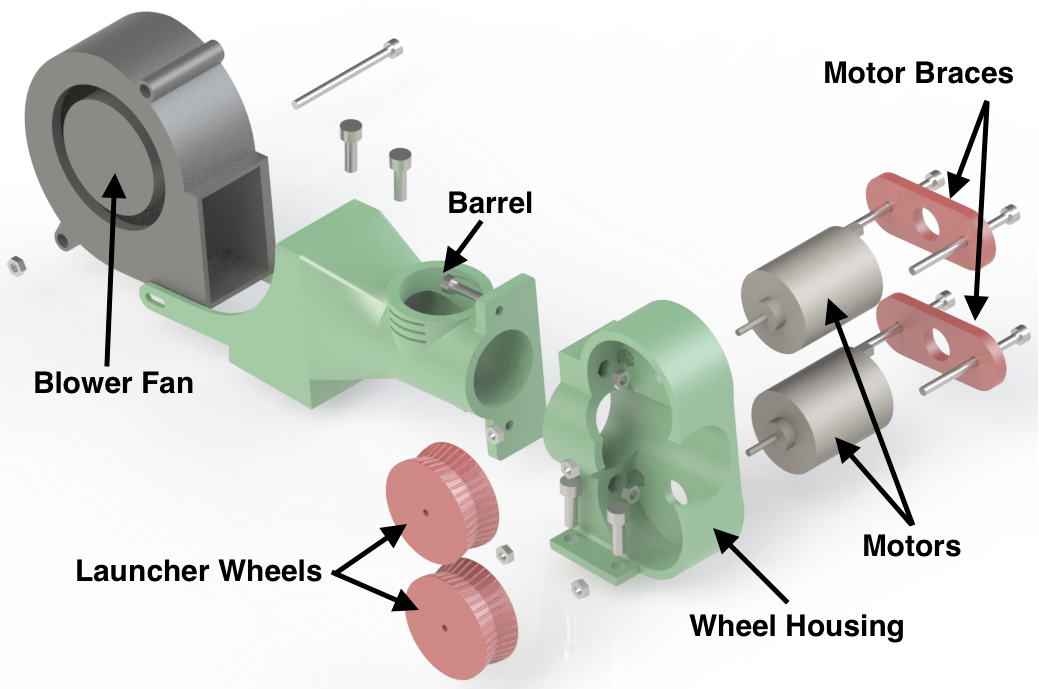
\includegraphics[width=6in, height=3.85in, keepaspectratio]{figures/shooter_explode.png}
	\caption{Shooting Mechanism -- Exploded View}	\label{fig:shooter_explode}
\end{figure}
\begin{figure}[H]   % [h] means here
	\centering 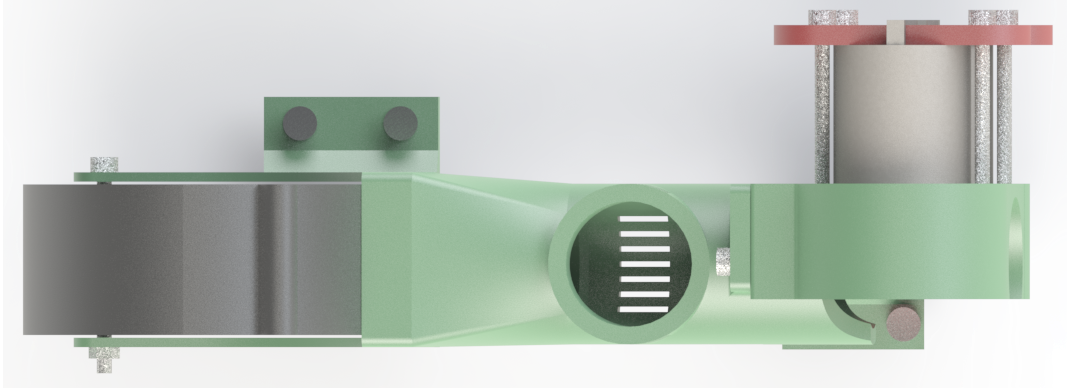
\includegraphics[width=6in, height=3.85in, keepaspectratio]{figures/shooter_top.png}
	\caption{Shooting Mechanism -- Top View}	\label{fig:shooter_top}
\end{figure}
\begin{figure}[H]   % [h] means here
	\centering 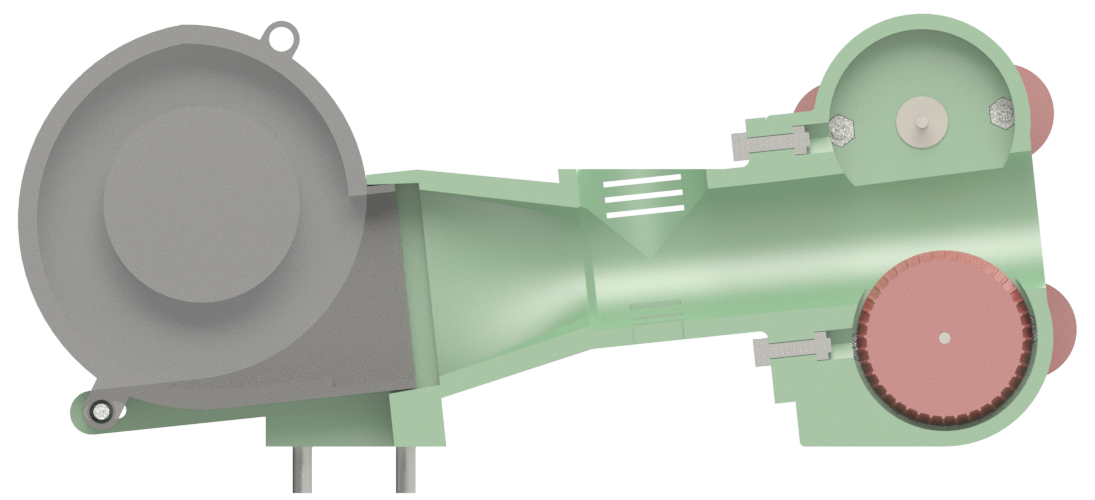
\includegraphics[width=6in, height=3.85in, keepaspectratio]{figures/shooter_xsec.png}
	\caption{Shooting Mechanism -- Cross Section View}	\label{fig:shooter_xsec}
\end{figure}




\section{Ball Hopper}

\section{Control Unit}